\documentclass[../../cjSOE.tex]{subfiles}

\begin{document}
%\begin{verbatimwrite}{../../insert_saving-and-uncert}
\subsection{Relation to a More Realistic Model}\label{subsec:robustness}

In this section, we relate our model's stylized treatment of uncertainty to the treatment in a related model with a much more realistic (but much less tractable) structure. Specifically, we use the model in \cite{cstwMPC} (henceforth 'CSTW'), which incorporates transitory and permanent idiosyncratic shocks {\it a la} \cite{friedmanATheory} calibrated to match empirical estimates of the magnitude of such household-level shocks in U.S.\ data.  We use that model to calculate a quantitative relationship between the central measures of uncertainty in the two models, and show how this helps provide an interpretation of the quantitative relationship of uncertainty to precautionary saving in our model.

The CSTW model specifies a household income process commonly used in the modern microfounded consumption literature.  Household income $y_{t}$ is determined by the aggregate wage rate $W_{t}$ and two idiosyncratic components, the permanent component $p_{t}$ and the transitory shock $\tshk_{t}$:
\begin{align}
  y_{t}=p_{t}\tshk_{t}{W}_{t}
\end{align}
The permanent component is subject to a shock $\pShk$:
\begin{align}
  p_{t}=p_{t-1}\permShk_{t}
\end{align}
while the transitory component is:
\begin{eqnarray}
  \xi_{t} & = & \mu \textrm{ with probability }\ \urate_{t}, %\label{eq:tran}
  \\ & = & (1-\tau_{t})\ell\theta_{t} \textrm{ with probability }\ 1-\urate_{t}, \nonumber
\end{eqnarray}
Here $\mu$ is the unemployment insurance payment when unemployed. $\tau_{t}$ is the rate of tax collected to pay unemployment benefits, $\ell$ is time worked per employee. $\permShk$ and $\theta$ are white noise shocks drawn from log normal distribution and $\mathbb{E}_{t}\permShk_{t+n}=\mathbb{E}_{t}\theta_{t+n}=1~\forall~n>0$. By changing the value of $\sigma^{2}_{\permShk}$ and $\sigma^{2}_{\theta}$, we change the degree of uncertainty faced by households.  Further details of the model are described in appendix A.7

CSTW find that in order for the model to generate a plausible distribution of wealth it is necessary to build in some form of \textit{ex ante} hetergogeneity; we follow them in assuming that the time preference rate is the locus of heterogeneity, and in calibrating the mean of the time discount factor to match the U.S.\ aggregate wealth to income ratio and the the spread of the time discount factor to match the wealth distribution among households in U.S.\ data.\footnote{The wealth to income ratio and wealth distribution data are obtained from the Survey of Consumer Finances.}

Following CSTW, we set the benchmark annual values of $\sigma_{\psi}^{2}$ and $\sigma^{2}_{\theta}$ to be $0.010$ and $0.010$.\footnote{Because CSTW is a quarterly model, these annual figures are translated to the corresponding quantities at the quarterly frequency.}  The growth impatience condition $\PatPGroAdj$ of the most patient agent restricts the maximum value of $\sigma_{\psi}^{2}$ we can choose.\footnote{Under this new model setup, the growth impatience condition needs to be modified to be $\PatPGroAdj = \frac{(\Discount \Rfree)^{1/\CRRA}\PLives}{\PGroAdj}$ were $\PGroAdj=\PGro/\mathbb{E}[\psi^{-1}]$.  We take care to make sure this condition is satisfied.}

% \begin{table}
%   % \ref{tab:Uncert}
%   \centering
%   \caption{Estimated Linear Relation Between Uncertainty and Saving}
%   \begin{tabular}{cccc}
%     \hline
%     & Slope & $R^2$ & max $\PatPGro$\\
%     \hline 
%     $\sigma_{\Psi}$ & 0.826 & 0.998 & 0.998\\
%     % & ($9.1\times10^{-3}$)***\\
%     $\sigma_{\theta}$ & 0.0111 & 0.989 & 0.996\\
%     % & ($3.1\times10^{-4}$)***\\
%     \hline
%   \end{tabular}
%   \begin{tablenotes}
%     \footnotesize
%   \item This table presents the relationship between the aggregate saving rate and the degree of income uncertainty. The first two columns show the slope and $R^2$ result from an OLS regression. The third column show the growth impatience factor of the most patient agent in the economy. The first row shows the result of an OLS regression of the aggregate saving rate on the variance of permanent income shocks $\sigma^{2}_{\psi}$. The second row shows the result of OLS regression between the aggregate saving rate and the variance  of transitory income shocks $\sigma^{2}_{\theta}$.  (No standard errors are reported because the simulation size was chosen to be large enough that the estimates are perfectly accurate for the displayed level of precision).
%   \end{tablenotes}
% \end{table}

% \begin{figure}[h]
%   % 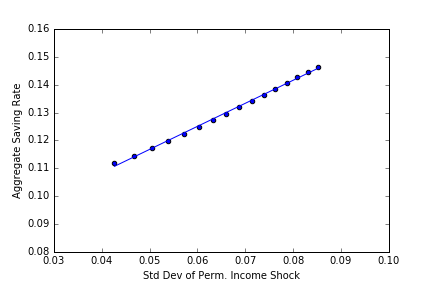
\includegraphics[scale=0.8]{\econtexRoot/LaTeX/Insertions/SavingVSPermShr_Youth_MPC_15.png}
%   \includegraphics[scale=0.8]{\econtexRoot/Figures/Uncertainty-and-the-Saving-Rate_PermShkVar}
%   \centering
%   \caption{Saving Rates at Different Levels of Permanent Shock Variance}
%   \label{figure:savings}
  
%   % 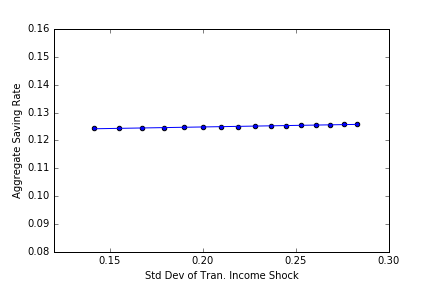
\includegraphics[scale=0.8]{\econtexRoot/LaTeX/Insertions/SavingVSTranShr_Youth_MPC_15.png}
%   \includegraphics[scale=0.8]{\econtexRoot/Figures/Uncertainty-and-the-Saving-Rate_TranShkVar}
%   \centering
%   \caption{Saving Rates at Different Levels of Transitory Shock Variance}
%   \label{figure:savingsTran}
% \end{figure}


\subsection{Translation}

%This paper's principal purpose is to provide a tractable model that yields analytical insights, because the model's treatment of income uncertainty is so stylized that it is not obvious how to translate its implications into empirically measurable phenomena.

Our unemployment shock is a permanent shock to income, so it is natural to interpret alternative values of $\urate$ as proxying for differences in the variance of permanent shocks $\sigma^{2}_{\pShk}$ in more realistic models. The difficulty is in knowing quantitatively how to translate alternative values of $\urate$ into the corresponding values of $\sigma^{2}_{\pShk}$.

To help with the translation we have constructed a rough bridge between the two models, as follows.  First, we set the parameters that the two models share, $\WGro, \EmpGro, \CRRA, \Rfree, \XperGro$, to the same values (the values reported in Table \ref{table:calibration}).  And we set the values of parameters unique to the CSTW model to their default values from that paper. 

Next, we find a value of $\urate$ at which the two models predict the same ratio of aggregate wealth to income, $\BRat$.  Here, the tractability of our model comes in handy; although the analytical function for $\BRat$ in terms of primitives\footnote{
  \begin{equation}
    \BRat = \left(      \frac{(\urate \EmpGro \WGro) (1-\kapShare)}{\EmpGro \WGro - \PLives \Pat}\right)\left[\frac{\PGro}{\Rfree}-\frac{1}{2-\LGro}+\MPCU\left(\frac{1+\PatPGro^{-\CRRA}-1}{\urate}\right)^{-\CRRA}\right]^{-1}
  \end{equation}}
is not analytically invertible, it is well-behaved (under appropriate parametrica assumptions) so that finding the $\urate$ for which $\BRat$ matches any particular value is numerically trivial.

For the case in hand, the CSTW model's value is $\bar{\BRat} = 2.56$ (matching the target from a 2010 JEDC symposium organized by \cite{djjKS} on solution methods for models of this class), and we calculate that our model generates $\BRat=2.565$ for $\urate \approx 0.01167\equiv\bar{\urate}$. 

The last step is to map deviations of the two variables, $\urate$ in the tractable model and $\sigma^{2}_{\psi}$ in the CSTW model, from their benchmark values in such a way that, locally, the mapped change in $\urate$ generates the same change in $\BRat$ as the corresponding change in $\sigma^{2}_{\psi}$.

It turns out that the relationships between steady-state net worth and our principal measures of uncertainty are not far from linear in either model; see \ref{fig:BandMho} and \ref{fig:BandPShockVar} for plots of the relation between $\BRat$ and each model's central measure of uncertainty ($\urate$ for the tractable model; $\sigma^{2}_{\pShk}$ for CSTW), over the range from half the benchmark value to the full benchmark value.  Because it is computationally expensive to calculate, the results from the CSTW model are presented at a set of points sufficient to reveal the shape of the underlying continuous function; because it is analytic, we can plot the function for the tractable model exactly.

Numerically, for a one-half reduction in the magnitude of the uncertainty measure, the two models predict a similar decline in the size of ne worth: In the tractable case, to a value about 0.71 times as large is the benchmark, and for the CSTW case to about 0.65 times the original value.

\begin{figure}
  \caption{Tractable Model}\label{fig:BandMho}
  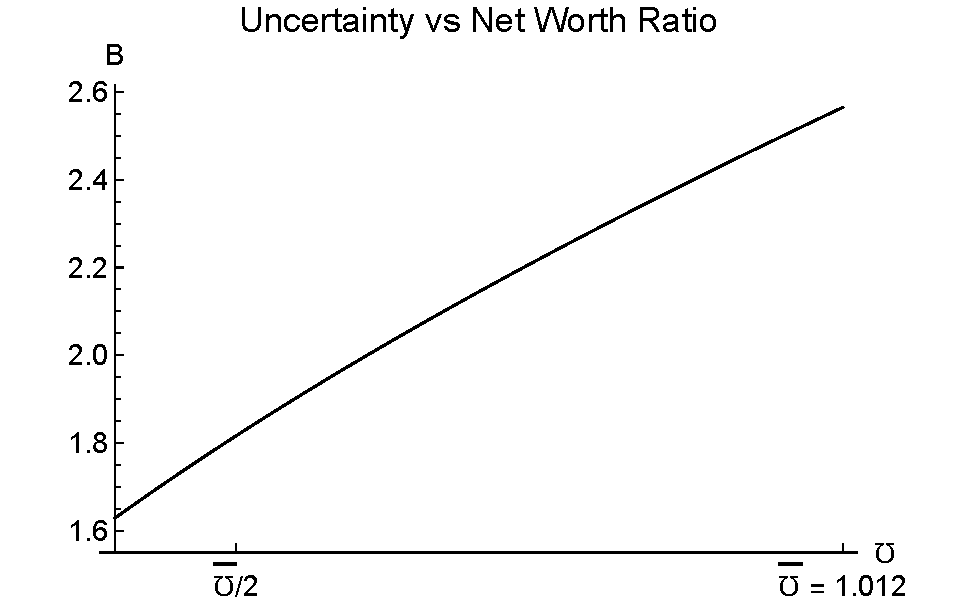
\includegraphics[width=5.5in]{\econtexRoot/Figures/BvsMho}
  \caption{CSTW Model}\label{fig:BandPShockVar}
  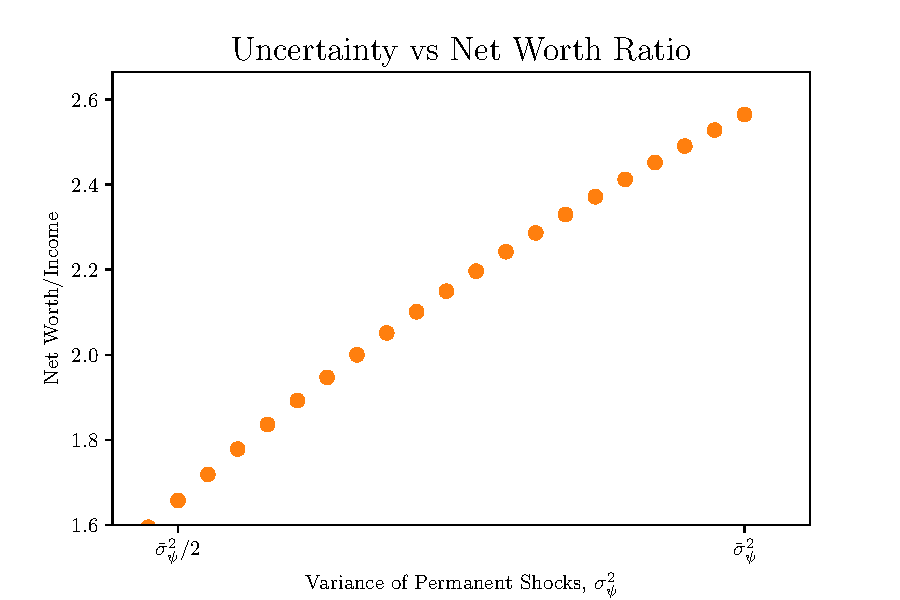
\includegraphics[width=6in]{\econtexRoot/Figures/Uncertainty-and-the-Saving-Rate-BvsPermShkVar}
\end{figure}

The two figures are encouragingly similar to each other over the corresponding ranges of their chief uncertainty measures, so we are comfortable in approximating the first order relationships in the vicinity of the target $\bar{\BRat}$ by 
\begin{eqnarray}
  \BRat_\text{tract}(\urate) & \approx & \bar{\BRat} + (\urate-\bar{\urate})\zeta_{\text{tract}} 
\end{eqnarray}
in the tractable model and 
\begin{eqnarray}
  \BRat_{\text{cstw}}(\sigma^{2}_{\pShk}) & \approx & \bar{\BRat} + (\sigma^{2}_{\pShk}-\bar{\sigma}^{2}_{\pShk})\zeta_{\text{cstw}} 
\end{eqnarray}
in the CSTW model.

Under these assumptions, there is some $\nu$ such that
\begin{eqnarray}
  \nu \left(\frac{d \BRatE_{\text{tract}}}{d \urate}\right) & \approx & \left(\frac{d \BRatE_{\text{cstw}}}{d \sigma^{2}_{\pShk}}\right) \\
  \nu \zeta_{\text{tract}} & \approx & \zeta_{\text{cstw}}
  \\ \nu & \approx & \zeta_{\text{cstw}}/\zeta_{\text{tract}}                                 \end{eqnarray}

% \zeta_{cstw}=504.94, \zeta_{tract}=128.49, so \nu=128.49/504.94=
When we undertake this exercise, we obtain a value of $\nu \approx 0.254$.  That is, the
conclusion is that a rough interpretation of a one unit change in $\urate$ is that it
is equivalent to a change of about $(1/4)$ as much in the measurable quantity $\sigma^{2}_{\pShk}$.

There is at present little evidence on the size of $\zeta_{cstw}$.  But recent years have seen a growing number of estimates of statistics like $\sigma^{2}_{\pShk}$ across countries.  Studies comparing small open economies with well-measured data both on saving rates and proxies for $\sigma^{2}_{\pShk}$ should be able to measure an empirical counterpart to $\zeta_{\text{cstw}}$, if variations in this statistic are in fact large enough to contribute importantly to the difference in saving rates across countries (as, for example, the IMF seems to believe is true [cite IMF advice to China to bolster its social safety net to encourage consumption]).

%\end{verbatimwrite}
%\subsection{Robustness Check}

In this section, we show that the positive relationship between income uncertainty and the aggregate saving rate holds in a model with more realistic settings than the basic tractable model. Specifically, we use the model in \cite{cstwMPC} (henceforth 'CSTW'), which incorporates transitory and permanent shocks {\it a la} \cite{friedmanATheory} calibrated to match empirical estimates of such shocks in U.S.\ data.  We use this model to calculate a quantitative relationship between uncertainty and precautionary saving.

In the basic model, the only uncertainty comes from the shock of becoming unemployed. Here household income $y_{t}$ is determined by the aggregate wage rate $W_{t}$ and two idiosyncratic components, the permanent component $p_{t}$ and the transitory shock $\tshk_{t}$:
\begin{align}
y_{t}=p_{t}\tshk_{t}{W}_{t}
\end{align}
The permanent component follows:
\begin{align}
p_{t}=p_{t-1}\permShk_{t}
\end{align}
The transitory component is:
\begin{eqnarray}
  \xi_{t} & = & \mu \textrm{ with probability }\ \urate_{t}, \label{eq:tran}
\\ & = & (1-\tau_{t})\ell\theta_{t} \textrm{ with probability }\ 1-\urate_{t}, \nonumber
\end{eqnarray}
Here $\mu$ is the unemployment insurance payment when unemployed. $\tau_{t}$ is the rate of tax collected to pay unemployment benefits, $\ell$ is time worked per employee. $\permShk$ and $\theta$ are white noise drawn from log normal distribution and $\mathbb{E}_{t}\permShk_{t+n}=\mathbb{E}_{t}\theta_{t+n}=1\forall n>0$. By changing the value of $\sigma_{\permShk}$ and $\sigma_{\theta}$. we change the degree of uncertainty faced by households.The details of the model are described in appendix A.7

%In this model, the economy consists of a continuum of households of mass one distributed on the unit interval. Households die with a constant probability $D=1-\PLives$ between periods. This is different from the baseline model in which households only face probability of dying after they become unemployed. Each household maximize expected discount utility from consumption:
%\begin{eqnarray}
%\max\mathbb{E}_{t}\sum_{n=0}^{\infty}(\PLives\beta)^{n}\util(\cFunc_{t+n})
%\end{eqnarray}
%The household consumption functions satisfies:
%\begin{eqnarray}
%v(m_{t}) & = & \max_{c_{t}} \mathbb{E}_{t}\sum_{n=0}^{\infty}(\PLives\beta)^{n}\util(\cFunc_{t+n}), \label{eq:tran}
%\\ \text{s.t.}, \nonumber
%\\a_{t} & = & m_{t}-\c(m_{t})
%\\k_{t+1} & = & \frac{a_{t}}{\PLives \permShk_{t+1}}
%\\m_{t+1} & = & (\DeprFac+r_{t})k_{t+1}+\tshk_{t+1}
%\\a_{t} & \geq & 0
%\end{eqnarray}
%The production function is Cobb-Douglass:
%\begin{align}
%\end{align}
%The aggregate wage rate $W_{t}$ is determined by the aggregate productivity $Z_{t}$, capital stock $K_{t}$, and the aggregate supply of labor $L_{t}$:
%\begin{align}
%\end{align}
%$L_{t}$ is driven by two aggregate shocks:
%\begin{align}
%\\P_{t}=P_{t-1}\Psi_{t}
%\end{align}
%where $P_{t}$ is aggregate permanent productivity, 	$\Psi_{t}$ is the aggregate permanent shock
%and $\Theta_{t}$ is the aggregate transitory shock.\footnote{Note that $\Psi$ is the capitalized version of the Greek letter $\psi$ used for the idiosyncratic permanent shock; similarly $\Theta$ is the capitalized $\theta$}

The parameters are calibrated at the same level as they are in CSTW except for aggregate productivity growth rate and individual productivity growth rate. In CSTW, there is no aggregate and individual productivity growth; here we allow aggregate productivity growth $G=1.015$, and individual productivity growth $X=1.01$.

CSTW find that in order for the model to generate a plausible distribution of wealth it is necessary to build in some form of \textit{ex ante} hetergogeneity; we follow them in assuming that the time preference rate is the locus of heterogeneity. We calibrate the mean of the time discount factor to match the U.S.\ aggregate wealth to income ratio and the distribution of the time discount factor to match the wealth distribution among households in U.S.\ data.\footnote{The wealth to income ratio and wealth distribution data are obtained from the Survey of Consumer Finances.}

%\begin{eqnarray}
%a_{t} & = & m_{t}-\c(m_{t}), \label{eq:cons1}
%\\ k_{t+1}& = & \frac{a_{t}}{\pLive \permShk_{t+1}}, \label{eq:cons2}
%\end{eqnarray}

Following CSTW, we set the benchmark value of $\sigma_{\psi}^{2}$ and $\sigma_{\theta}^{2}$ to be $0.010\times4/11$ and $0.010\times4$. Under these new model settings, the growth impatience condition needs to be modified to be:

\begin{align}
	\PatPGroAdj = \frac{(\Discount \Rfree)^{1/\CRRA}\PLives}{\PGroAdj}
\end{align}
Where $\PGroAdj=\PGro \acute{\psi}$ and $\acute{\psi}\equiv (\mathbb{E}[\psi^{-1}])^{-1}$. By computing aggregate saving rate while increasing $\sigma_{\psi}^{2}$ and $\sigma_{\theta}^{2}$,  we derive the relationship between aggregate saving rate and the degree of uncertainty. Increasing $\sigma_{\psi}^{2}$ will also cause $\PGroAdj$ to increase. Agents with different $\beta$ have different $\PGroAdj$. The growth impatience condition $\PGroAdj<1$ of the most patient agent restricts the maximum value of $\sigma_{\psi}^{2}$ we can choose. Here we allow $\sigma_{\psi}^{2}$ and $\sigma_{\theta}^{2}$ to move from half of their benchmark values to twice the benchmark value.  Figure \ref{figure:savings} shows how the aggregate saving rate changes with $\sigma_{\psi}$. The first row in Table 2 reports the slope and $R^2$ calculated from OLS regression between the aggregate saving rate and the standard deviation of the permanent income shock. Under the model calibration, aggregate saving rate is almost perfectly correlated with the standard deviation of $\sigma_{\psi}$: adding 0.01 to $\sigma_{\psi}$ will cause the aggregate savings rate to rise about 0.83 percent. Figure \ref{figure:savingsTran} shows how the aggregate saving rate varies with the standard deviation of the transitory income shock. The regression result is reported in the second row of Table 2. The impact of transitory uncertainty is much smaller than the impact of permanent uncertainty. Increasing  $\sigma_{\theta}$ by 0.01 will cause the aggregate saving rate to increase by 0.011 percent. The last column reports the growth impatience factor of the most patient agent when $\sigma_{\psi}^{2}$ reaches its upper limit in each of the two exercises. We can see that the growth impatience condition is well satisfied in both exercises.
%\PatPGro
\begin{table}
	\centerline{\bf Table 2}
	\label{tab:Uncert}
	\begin{center}
		\begin{tabular}{ c c c c }
			\hline
			~ & Slope & $R^2$ & max $\PatPGro$\\
			\hline
			\multirow{2}{4em}{$\sigma_{\Psi}$} & 0.826 & \multirow{2}{*}{0.998} & \multirow{2}{4em}{0.998}\\
			& ($9.1\times10^{-3}$)***\\
			\multirow{2}{4em}{$\sigma_{\theta}$} & 0.0111 & \multirow{2}{*}{0.989} & \multirow{2}{4em}{0.996}\\
			& ($3.1\times10^{-4}$)***\\
			\hline
		\end{tabular}
		\\
	\end{center}
	\begin{tablenotes}
		\small
		\item Table 2 presents the correlation between the aggregate saving rate and the degree of income uncertainty. The first two columns show the slope and $R^2$ result from OLS regression. The third column show the growth impatience factor of the most patient agent in the economy. The first row shows the result of OLS regression between the aggregate saving rate and the standard deviation of permanent income shocks $\sigma_{\psi}$. The second row shows the result of OLS regression between the aggregate saving rate and the standard deviation of transitory income shocks $\sigma_{\theta}$. Standard errors are reported in parenthesis. ***represents significance level of 0.01.
	\end{tablenotes}
\end{table}

\begin{figure}[h]
	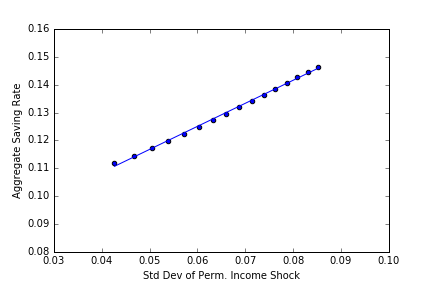
\includegraphics[scale=0.8]{\econtexRoot/LaTeX/Insertions/SavingVSPermShr_Youth_MPC_15.png}
	\centering
	\caption{Change in Savings Following increasing in Permanent Income Uncertainty}
	\label{figure:savings}

	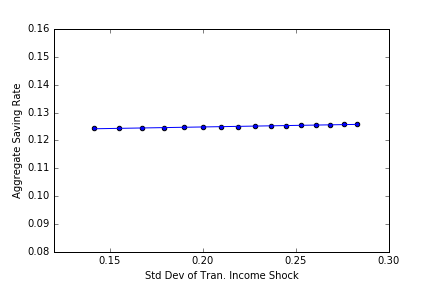
\includegraphics[scale=0.8]{\econtexRoot/LaTeX/Insertions/SavingVSTranShr_Youth_MPC_15.png}
	\centering
	\caption{Change in Savings Following increasing in Transitory Income Uncertainty}
	\label{figure:savingsTran}
\end{figure}



%\bibliographystyle{ier}
%\bibliography{economics}
\end{document}
